%%%%%%%%%%%%%%%%%%%%%%%%%%%%%%%%%%%%%%%%%
% Jacobs Landscape Poster
% LaTeX Template
% Version 1.1 (14/06/14)
%
% Created by:
% Computational Physics and Biophysics Group, Jacobs University
% https://teamwork.jacobs-university.de:8443/confluence/display/CoPandBiG/LaTeX+Poster
% 
% Further modified by:
% Nathaniel Johnston (nathaniel@njohnston.ca)
%
% This template has been downloaded from:
% http://www.LaTeXTemplates.com
%
% License:
% CC BY-NC-SA 3.0 (http://creativecommons.org/licenses/by-nc-sa/3.0/)
%
%%%%%%%%%%%%%%%%%%%%%%%%%%%%%%%%%%%%%%%%%

%----------------------------------------------------------------------------------------
%	PACKAGES AND OTHER DOCUMENT CONFIGURATIONS
%----------------------------------------------------------------------------------------

\documentclass[final]{beamer}

\usepackage[utf8]{inputenc}
\usepackage[T1]{fontenc}
\usepackage{url}
\usepackage{adjustbox}
\usepackage{float}
\usepackage{smartdiagram}
\usepackage{amsmath}
\usepackage{amssymb}
\usepackage{tikz}
\usetikzlibrary{shapes.geometric, arrows}
\usetikzlibrary{positioning}
\tikzstyle{io} = [
rectangle,
rounded corners,
minimum width=3cm,
minimum height=1cm,
text centered,
draw=black,
text width=3cm]

\tikzstyle{process} = [
rectangle,
minimum width=3cm,
minimum height=1cm,
text centered,
text width=3.5cm,
draw=black,
fill=gray!30]

\tikzstyle{arrow} = [thick,->,>=stealth]

\usepackage{hyperref}

\usepackage[scale=0.68,size=a1]{beamerposter} % Use the beamerposter package for laying out the poster

\usetheme{confposter} % Use the confposter theme supplied with this template

\setbeamercolor{block title}{fg=ngreen,bg=white} % Colors of the block titles
\setbeamercolor{block body}{fg=black,bg=white} % Colors of the body of blocks
\setbeamercolor{block alerted title}{fg=white,bg=dblue!70} % Colors of the highlighted block titles
\setbeamercolor{block alerted body}{fg=black,bg=dblue!10} % Colors of the body of highlighted blocks
% Many more colors are available for use in beamerthemeconfposter.sty

%-----------------------------------------------------------
% Define the column widths and overall poster size
% To set effective sepwid, onecolwid and twocolwid values, first choose how many columns you want and how much separation you want between columns
% In this template, the separation width chosen is 0.024 of the paper width and a 4-column layout
% onecolwid should therefore be (1-(# of columns+1)*sepwid)/# of columns e.g. (1-(4+1)*0.024)/4 = 0.22
% Set twocolwid to be (2*onecolwid)+sepwid = 0.464
% Set threecolwid to be (3*onecolwid)+2*sepwid = 0.708

\newlength{\sepwid}
\newlength{\onecolwid}
\newlength{\twocolwid}
\newlength{\threecolwid}
\setlength{\paperwidth}{33.11in} % A0 width: 46.8in
\setlength{\paperheight}{23.39in} % A0 height: 33.1in
\setlength{\sepwid}{0.024\paperwidth} % Separation width (white space) between columns
\setlength{\onecolwid}{0.22\paperwidth} % Width of one column
\setlength{\twocolwid}{0.464\paperwidth} % Width of two columns
\setlength{\threecolwid}{0.708\paperwidth} % Width of three columns
\setlength{\topmargin}{-0.5in} % Reduce the top margin size

\DeclareFontShape{OMX}{cmex}{m}{n}{
  <-7.5> cmex7
  <7.5-8.5> cmex8
  <8.5-9.5> cmex9
  <9.5-> cmex10
}{}

\SetSymbolFont{largesymbols}{normal}{OMX}{cmex}{m}{n}
\SetSymbolFont{largesymbols}{bold}  {OMX}{cmex}{m}{n}
%-----------------------------------------------------------

\usepackage{graphicx}  % Required for including images

\usepackage{booktabs} % Top and bottom rules for tables

%----------------------------------------------------------------------------------------
%	BIBLIOGRAPHY SECTION 
%----------------------------------------------------------------------------------------

\usepackage{biblatex}
\addbibresource{cite.bib}

%----------------------------------------------------------------------------------------
%	Definitions
%----------------------------------------------------------------------------------------

\renewcommand{\vec}[1]{\mathbf{#1}}
\renewcommand{\L}{\mathcal{L}}
\newcommand{\D}{\mathcal{D}}
\newcommand{\Exp}{\mathbb{E}}
\newcommand{\KL}[2]{\mathrm{KL}\left(\,#1\,\,||\,\,#2\,\right)}
\newcommand{\dee}{\mathrm{d}}
\newcommand{\Q}{\mathcal{Q}}
\newcommand{\N}{\mathcal{N}}
\newcommand{\diag}{\mathrm{diag}}
\newcommand{\Reals}{\mathbb{R}}
\newcommand{\F}{\mathcal{F}}
\newcommand{\pd}[2]{\frac{\partial #1}{\partial #2}}

\DeclareMathOperator*{\argmax}{arg\,max}
\DeclareMathOperator*{\argmin}{arg\,min}

%----------------------------------------------------------------------------------------
%	TITLE SECTION 
%----------------------------------------------------------------------------------------

\title{Compression without Quantization} 

\author{Gergely Flamich, Marton Havasi, Jos\'e Miguel Hern\'andez-Lobato \\
        5 June 2019} % Author(s) 

%\institute{} % Institution(s)

%----------------------------------------------------------------------------------------

\begin{document}

\setbeamertemplate{caption}[numbered]

\addtobeamertemplate{headline}{} 
{
\begin{tikzpicture}[remember picture,overlay] 
\node [shift={(-10 cm,-2.5
cm)}] at (current page.north east) {\includegraphics[height=7cm]{../img/poster/uni_logo.png}}; 
\end{tikzpicture} 
}
\vspace{-5cm}

\addtobeamertemplate{block end}{}{\vspace*{2ex}} % White space under blocks
\addtobeamertemplate{block alerted end}{}{\vspace*{2ex}} % White space under highlighted (alert) blocks

\setlength{\belowcaptionskip}{2ex} % White space under figures
\setlength\belowdisplayshortskip{2ex} % White space under equations

\begin{frame}[t] % The whole poster is enclosed in one beamer frame

\begin{columns}[t] % The whole poster consists of three major columns, the second of which is split into two columns twice - the [t] option aligns each column's content to the top

\begin{column}{\sepwid}\end{column} % Empty spacer column

\begin{column}{\onecolwid} % The first column

%----------------------------------------------------------------------------------------
%	OBJECTIVES
%----------------------------------------------------------------------------------------

\begin{alertblock}{Objectives}

In this work we propose a novel lossy image compression technique based on
MIRACLE \cite{havasi2018minimal}, that is:
\begin{itemize}
\item \textbf{principled:} our method is based on the MDL principle
  \cite{hinton1993keeping}, as we
  l earn encoding and decoding distributions over a latent representation of
  images, which then allows us to use Arithmetic Coding to compress a random
  latent sample.
\item \textbf{efficient:} with our method we can compress images close to their
  information-theoretical limit (in the bits-back sense \cite{hinton1993keeping}).
\item \textbf{differentiable:} in contrast to previous work, our method does not
  require quantization (which is non-differentiable) for compression, hence our
  system can be trained end-to-end.
\end{itemize}

\end{alertblock}

%----------------------------------------------------------------------------------------
%	INTRODUCTION
%----------------------------------------------------------------------------------------

\begin{block}{Introduction}
Based on earlier work on lossy image compression using VAEs by Ball\'e
\cite{balle2018variational}, we show that their architecture when interpreted in
the MIRACLE framework corresponds to a Hieararchical VAE \cite{sonderby2016train}.
We use the hierarchical structure reported in \cite{balle2018variational}, but
unlike them, we omit the quantization step and use diagonal Gaussians as the
latent priors $p(\vec{z})$ and posteriors $q(vec{z} \mid \vec{x})$.
We train on the CLIC 2018 dataset \cite{clic2018} using the ELBO for Gaussian
likelihood on the data:
\begin{equation}
  \L = \Exp_q[\log p(\D \mid \vec{z})] + \KL{q(\vec{z} \mid \D)}{p(\vec{z})}
\end{equation}
, which equivalent
to optimizing for the PSNR \cite{psnr} as a perceptual metric. 

\noindent
To accommodate variable size images, we use a fully convolutional
architecture, meaning we will have a variable size latent space. This is
natural, as we would want a larger latent representation for larger images.

\end{block}

%----------------------------------------------------------------------------------------

\end{column} % End of the first column

\begin{column}{\sepwid}\end{column} % Empty spacer column

\begin{column}{\twocolwid} % Begin a column which is two columns wide (column 2)

%----------------------------------------------------------------------------------------
%	IMPORTANT RESULT
%----------------------------------------------------------------------------------------

\begin{block}{Results}

\begin{figure}
\centering
\begin{minipage}[t]{.47\textwidth}
  \centering
  \includegraphics[width=\textwidth]{../img/poster/original.png} 
  \caption{haha}
  \label{fig:original_tattoo}
\end{minipage}%
\hfill
\begin{minipage}[t]{.47\textwidth}
  \centering
  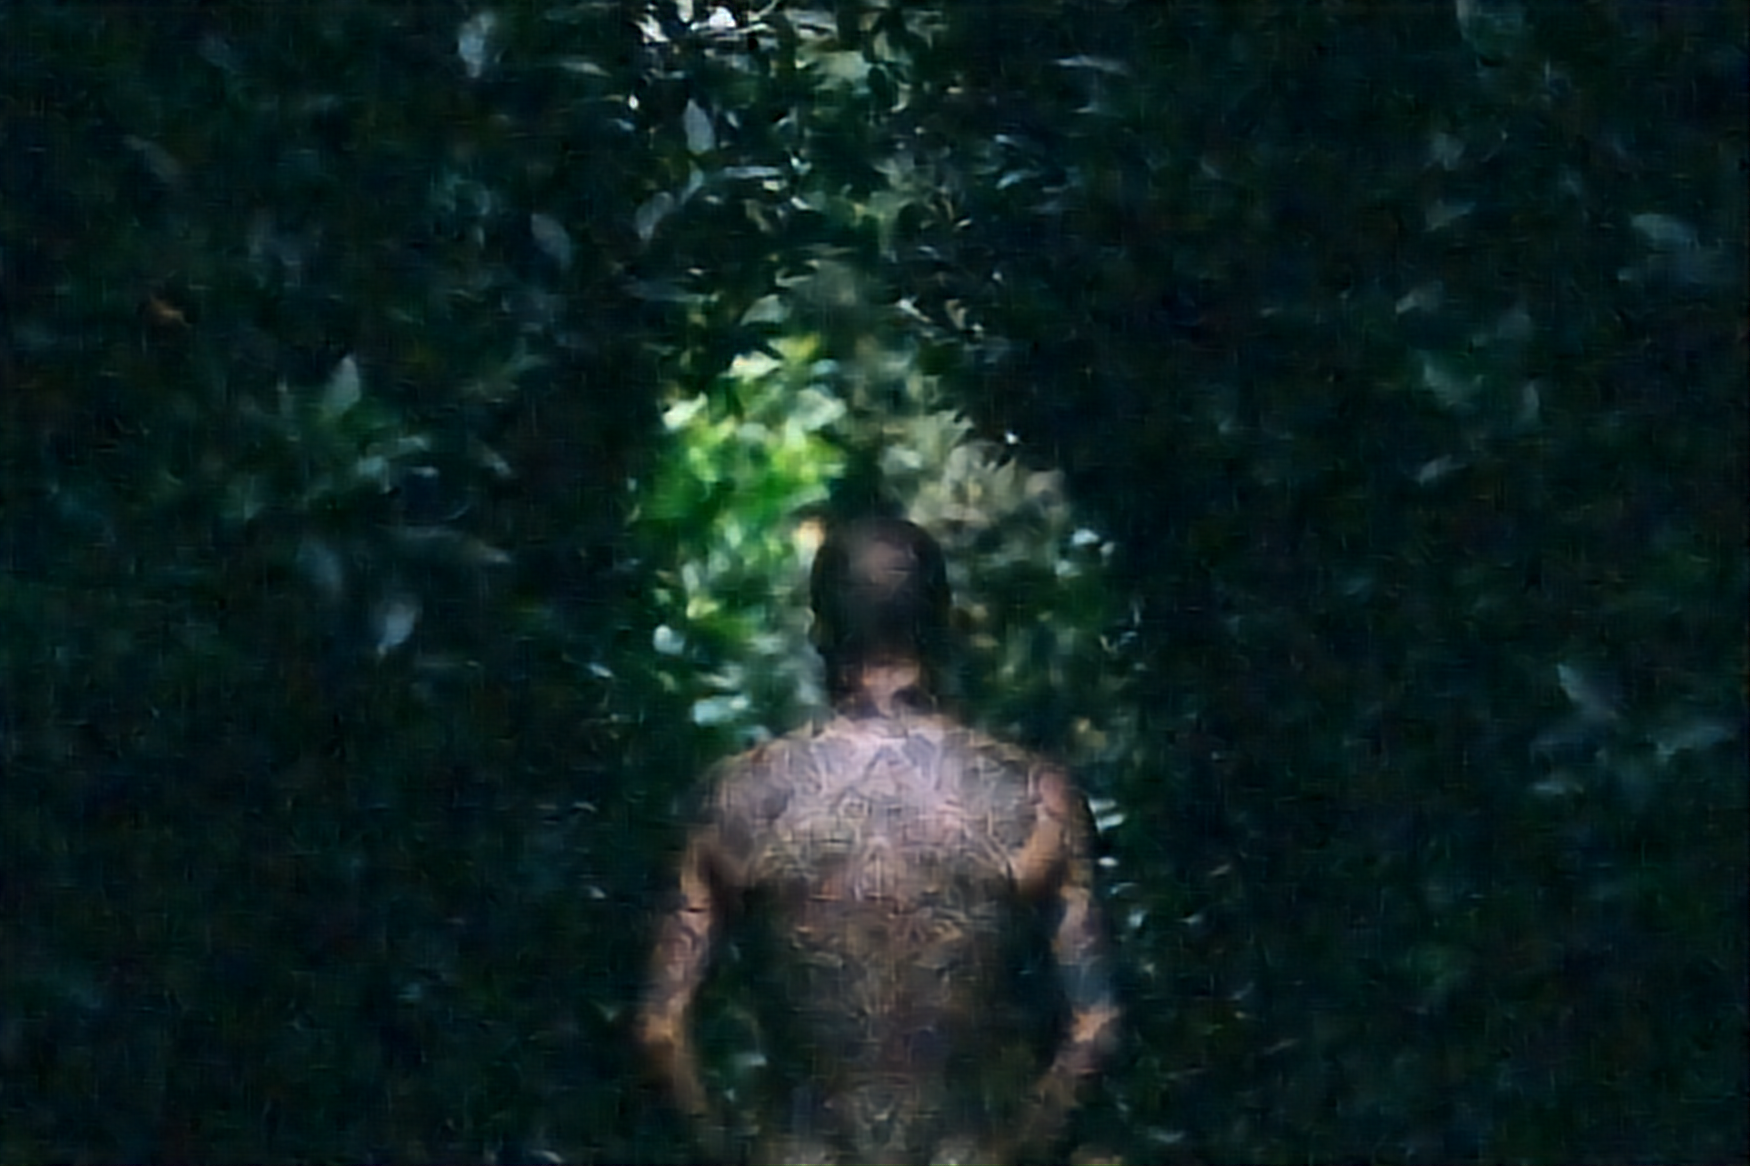
\includegraphics[width=\textwidth]{../img/poster/gauss_gauss.png}
  \caption{hehe}  
  \label{fig:reconstructed_tattoo}
\end{minipage}
\end{figure}

\end{block}

%----------------------------------------------------------------------------------------

\begin{columns}[t,totalwidth=\twocolwid] % Split up the two columns wide column again

\begin{column}{\onecolwid} % The first column within column 2 (column 2.1)

%----------------------------------------------------------------------------------------
%	MATHEMATICAL SECTION
%----------------------------------------------------------------------------------------

\begin{block}{Architecture}
  \begin{figure}[H]
    \centering
    \includegraphics[width=\textwidth]{../img/poster/uni_logo.png}
    \label{fig:architecture}
  \end{figure}

  \noindent
  For a single training example $\vec{x}$, our encoding distribution $q(\vec{z} \mid \vec{x})$
  Factorizes as $q(\vec{z}_1 \mid \vec{x})q(\vec{z}_2 \mid \vec{z}_1)$ where
  \begin{gather*}
    q(\vec{z}_1 \mid \vec{x}) = \N(\vec{z}_1 \mid \mu^{(e)}_1(\vec{x}),
    \sigma^{(e)}_1(\vec{x})) \\
    q(\vec{z}_2 \mid \vec{z}_1) = \N(\vec{z}_2 \mid \mu^{(e)}_2(\vec{z}_1),
    \sigma^{(e)}_2(\vec{z}_1)).
  \end{gather*}
  The generative model / decoding distribution $p(\vec{z},
  \vec{x})$ factorizes as $p(\vec{z}_1)p(\vec{z}_2\mid \vec{z}_1)p(\vec{x} \mid
  \vec{z}_1)$ where
  \begin{gather*}
    p(\vec{z}_2) = \N(\vec{z}_2 \mid \vec{0}, I) \\
    p(\vec{z}_1 \mid \vec{z}_2) = \N(\vec{z}_1 \mid \mu^{(d)}_2(\vec{z}_2),
    \sigma^{(d)}_2(\vec{z}_2)) \\ 
    p(\vec{x} \mid \vec{z}_1) = \N(\vec{x} \mid \mu^{(d)}_1(\vec{z}_1), I). 
  \end{gather*}
  The $\mu^{(\cdot)}_i(\cdot), \sigma^{(\cdot)}_i(\cdot)$ are given by the layers
  of the network as in Figure \ref{fig:architecture}.
  We use General Divisive Normalization \cite{balle2016end} as the activation
\begin{equation}
  a^{(k + 1)}_i(m, n) = \frac{u^{(k)}_i(m, n)}{\sqrt{\beta^{(k)}_i + \sum_j \gamma^{(k)}_jw^{(k)}_j(m, n)^2}}
\end{equation}

\end{block}

%----------------------------------------------------------------------------------------

\end{column} % End of column 2.1

\begin{column}{\onecolwid} % The second column within column 2 (column 2.2)

%----------------------------------------------------------------------------------------
%	RESULTS
%----------------------------------------------------------------------------------------

\begin{block}{Coding}

\end{block}

%----------------------------------------------------------------------------------------

\end{column} % End of column 2.2

\end{columns} % End of the split of column 2

\end{column} % End of the second column

\begin{column}{\sepwid}\end{column} % Empty spacer column

\begin{column}{\onecolwid} % The third column

%----------------------------------------------------------------------------------------
%	CONCLUSION
%----------------------------------------------------------------------------------------

\begin{block}{Conclusion}

Nunc tempus venenatis facilisis. \textbf{Curabitur suscipit} consequat eros non porttitor. Sed a massa dolor, id ornare enim. Fusce quis massa dictum tortor \textbf{tincidunt mattis}. Donec quam est, lobortis quis pretium at, laoreet scelerisque lacus. Nam quis odio enim, in molestie libero. Vivamus cursus mi at \textit{nulla elementum sollicitudin}.

\end{block}

%----------------------------------------------------------------------------------------
%	ADDITIONAL INFORMATION
%----------------------------------------------------------------------------------------

%----------------------------------------------------------------------------------------
%	REFERENCES
%----------------------------------------------------------------------------------------

\begin{block}{References}

\nocite{*} % Insert publications even if they are not cited in the poster
\small{
\printbibliography\vspace{0.75in}}

\end{block}

\end{column} % End of the third column

\end{columns} % End of all the columns in the poster

\end{frame} % End of the enclosing frame

\end{document}

